\documentclass[../main.tex]{subfiles}
\graphicspath{{\subfix{../images/}}}
\begin{document}


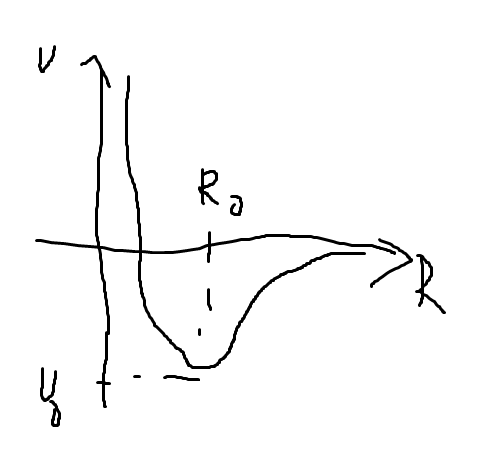
\includegraphics[width=0.75\linewidth]{images/potencial.png}

Provedeme taylorův rozvoj v $R_0$

\begin{equation}
    U(R) = U(R_0) + \frac{d U}{dR}(R_0)\frac{R-R_0}{1!} + \dots
\end{equation}

První derivace je 0, a zavádíme značení $(R - R_0) = x$, druhou derivaci označíme jako $\beta$ a třetí jako $-2\gamma$.

Máme
\begin{equation}
    U - U_0 = \frac{1}{2}\beta x^2 - \frac{1}{3} \gamma x^2
\end{equation}

Síla je pak jako 
\begin{equation}
    \vec{F} = - \frac{d U}{dx} = -\beta x + \gamma x^2
\end{equation}


\subsection{Iontové krystaly}
Pro 2 N iontů

Mezi ionty máme
$U(R) \frac{A}{R^m} - \frac{B}{R^n} $
To je energie mezi i-tým a k=tým iontem

Vzdálenost je $M_{ik} = q_{ik}R$

Definujeme $B \equiv \pm e^2, n\equiv 1$

Dáme do energie 
\begin{equation}
    U_{ik} = \frac{a}{R^m} \frac{1}{q^m_{ik}} - \frac{e^2}{R} \frac{\pm1}{q_{ik}}
\end{equation}

Na jeden atom působí pak síla 
\begin{equation}
    U_i = \sum_{k} U_{ik} = \frac{1}{R^m} a \sum_k \frac{1}{q^m_{ik}}
    - \frac{e^2}{R} \sum_k \frac{(\pm 1)^k}{q_{ik}}    
\end{equation}

Madelungova konstanta
\begin{equation}
   \alpha = \sum_k \frac{(\pm 1)^k}{q_{ik}} 
\end{equation}

Pokud bychom spočítali Madelungovu konstantu pro řetízek atomů dostaneme 
\begin{equation}
    \alpha = \sum_k \frac{(\pm 1)^k}{q_{ik}} = 
    2 \sum_{k=0}^\infty \frac{(\pm 1)^{k-1}}{k} =
    2\left(1 - 1/2 + 1/3 - 1/4 + \dots\right)=
    2 \ln 2 \approx 1.386 
\end{equation}

Což je srovnatelné s naměřenými hodnotami, například
\begin{equation}
    \alpha_{NaCl} = 1,748
\end{equation}

\begin{equation}
    \alpha_{CsCl} = 1,763
\end{equation}

\begin{equation}
    \alpha_{ZnS} = 1,638
\end{equation}

Energie krystalu je pak 

\begin{equation}
    U = \frac{1}{2} 2 N u_i = N u_i
\end{equation}
\begin{equation}
    U = N(\frac{A}{R^m} - \frac{\alpha e^2}{R})
\end{equation}

\begin{equation}
    \left(\frac{dU}{dR}\right)_{R_0} = N \left(\frac{du}{dR}\right)_{R_0} = 0
\end{equation}
Dostáváme vztah
\begin{equation}
    \frac{A}{R^m_0} = \frac{\alpha e^2}{m R_0}
\end{equation}

\begin{equation}
    U_0 = N u_0 = \frac{-N e^2 \alpha}{R_0} \left(1-\frac{1}{m}\right)
\end{equation}

\subsection{Kovalentní vazba}
$H_2$ (Heitler, London)

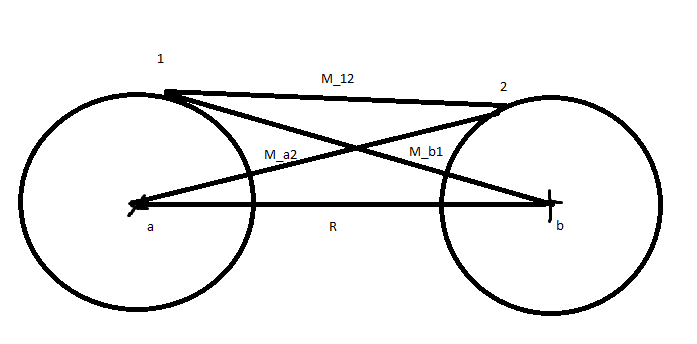
\includegraphics[width=\linewidth]{images/kovalentni_vazba.png}

$a_0$ je Bohrův poloměr

Z kvantovky máme 
\begin{equation}
    \psi_a = \frac{1}{\sqrt{\pi a_{0}^3}} \exp \left(- \frac{r_{a1}}{a_0}\right) \equiv \psi_a(1)
\end{equation}

\begin{equation}
    \psi_b = \frac{1}{\sqrt{\pi a_{0}^3}} \exp \left(- \frac{r_{b2}}{a_0}\right) \equiv \psi_b(2)
\end{equation}

Z principu nerozlišitelnosti máme $1 \leftrightarrow 2$

Hamiltonián má tvar 
\begin{equation}
    \mathcal{H}_a^0 = - \frac{\hbar^2}{2m} \nabla_1^2 - \frac{e^2}{r_{a2}}
\end{equation}
\begin{equation}
    \mathcal{H}_b^0 = - \frac{\hbar^2}{2m} \nabla_2^2 - \frac{e^2}{r_{b1}}
\end{equation}

Z principu nerozlišitelnosti 

\begin{equation}
    \mathcal{H}_a^0 = - \frac{\hbar^2}{2m} \nabla_1^2 - \frac{e^2}{r_{a1}}
\end{equation}
\begin{equation}
    \mathcal{H}_b^0 = - \frac{\hbar^2}{2m} \nabla_2^2 - \frac{e^2}{r_{b2}}
\end{equation}


Poruchovou teorií máme (0. aproximace)
\begin{equation}
    \mathcal{H}_a^0 \psi_a(1)= \varepsilon_0 \psi_a(1) 
\end{equation}
\begin{equation}
    \mathcal{H}_b^0 \psi_b(2) = \varepsilon_0 \psi_b(2)
\end{equation}

kde $\varepsilon_0 = \frac{- e^2}{2a_0}$


2 nezávislé atomy 
\begin{equation}
    \left[ \mathcal{H}_a^0 + \mathcal{H_a^0} \right] \psi(1,2) = E \psi(1,2)
\end{equation}

\begin{equation}
    \psi(1,2) = \psi_a(1)\psi_b(2)
\end{equation}

\begin{equation}
    E = 2 \varepsilon_0
\end{equation}

Pokud uděláme 1. aproximaci máme 
\begin{equation}
    E = 2 \varepsilon_0 + \epsilon
\end{equation}

\begin{equation}
    \Phi = c_1 \psi_a(1)\psi_b(2) + c_2 \psi_a(2)\psi_b(1)
\end{equation}

\begin{equation}
    W(1,2) = \frac{e^2}{r_{12}} + \frac{-e^2}{r_{a1}} + \frac{-e^2}{r_{b2}}
\end{equation}

Pak máme 
\begin{equation}
    \left[ \mathcal{H}_a^0 + \mathcal{H_a^0} + W(1,2) \right] \Phi  = E \Phi
\end{equation}

dostaneme
\begin{equation}
    \psi^0_S (1,2) = \psi_a(1) \psi_b(2) + \psi_a(2) \psi_b(1), \text{symetrické}
\end{equation}


\begin{equation}
    \psi^0_{AS} (1,2) = \psi_a(1) \psi_b(2) - \psi_a(2) \psi_b(1), \text{äntisymetrické}
\end{equation}

Z principu nerozlišitelnosti

\begin{equation}
    \psi^0_S (1,2) = \psi^0_S (2,1)
\end{equation}
\begin{equation}
    \psi^0_{AS} (1,2) = - \psi^0_{AS} (2,1)
\end{equation}

Z toho odvozujeme že \begin{equation}
    \psi^0_{S} 
\end{equation}
odpovídá singletnímu stavu

\begin{equation}
    \psi^0_{AS}
\end{equation}
odpovídá tripletnímu stavu. 


Pro energii máme 
\begin{equation}
    E = 2 \varepsilon_0 + \epsilon_s
\end{equation}
a 

\begin{equation}
    E = 2 \varepsilon_0 + \epsilon_{as}
\end{equation}

kde 

\begin{equation}
    \epsilon_s = \frac{K+A}{1+S^2}
\end{equation}

\begin{equation}
    \epsilon_{as} = \frac{K - A}{1 - S^2}
\end{equation}

\begin{equation}
    K = \int \psi_a(1) \psi_b(2)W(1,2) d\tau_1 d\tau_2
\end{equation}

\begin{equation}
    A = \int \psi_a(1) \psi_b(1) \psi_a(2) \psi_b(2)W(1,2) d\tau_1 d\tau_2
\end{equation}

\begin{equation}
    S^2 = \int \psi_a(1) \psi_b(1)\psi_a(2) \psi_b(2) d\tau_1 d\tau_2
\end{equation}










\end{document}